\documentclass[12pt]{article}
\usepackage{geometry}                % See geometry.pdf to learn the layout options. There are lots.
\geometry{letterpaper}                   % ... or a4paper or a5paper or ... 
%\geometry{landscape}                % Activate for for rotated page geometry
%\usepackage[parfill]{parskip}    % Activate to begin paragraphs with an empty line rather than an indent
\usepackage{graphicx}
\usepackage{amssymb}
\usepackage{subfig}
\usepackage{multirow}
\usepackage[margin=20pt, font=small,labelfont=sc, labelsep=endash]{caption}
\usepackage{pstricks, pst-node,pst-tree}


\title{Analysis of loadings}
\author{Wesley Brooks}
\date{}                                           % Activate to display a given date or no date

\usepackage{Sweave}
\begin{document}
\setkeys{Gin}{width=0.9\textwidth}    %make figures a bit wider than the Sweave default.
\maketitle



















The next block prints a table of the proportion of total phosphorus loading due to each class of event at each site\\


% latex table generated in R 2.13.0 by xtable 1.5-6 package
% Sun Aug 14 16:56:26 2011
\begin{table}[h]
\begin{center}
\begin{tabular}{lccc}
  & snowmelt-driven & early post-snow & late post-snow \\ 
  \hline
eagle & 27.0\% & 29.1\% & 43.9\% \\ 
  joosvalley & 26.9\% & 20.5\% & 52.6\% \\ 
  otter & 35.4\% & 20.5\% & 44.1\% \\ 
  brewery & 32.8\% & 4.5\% & 62.7\% \\ 
  \end{tabular}
\caption{Proportion of total suspended solids loading contributed by each type of event}
\label{tab:stot}
\end{center}
\end{table}
% latex table generated in R 2.13.0 by xtable 1.5-6 package
% Sun Aug 14 16:56:26 2011
\begin{table}[h]
\begin{center}
\begin{tabular}{lccc}
  & snowmelt-driven & early post-snow & late post-snow \\ 
  \hline
eagle & 32.8\% & 22.9\% & 44.2\% \\ 
  joosvalley & 36.4\% & 16.9\% & 46.7\% \\ 
  otter & 46.5\% & 16.6\% & 36.9\% \\ 
  brewery & 49.6\% & 4.5\% & 45.9\% \\ 
  \end{tabular}
\caption{Proportion of total phosphorus loading contributed by each type of event}
\label{tab:ptot}
\end{center}
\end{table}










Produce plots of the proportion of the suspended solids and phosphorus (both total loading and stormflow loading) that is contributed by each class of event at each stream site:\\



\begin{figure}[h!]
    \begin{center}
\includegraphics{loadings-fig2}
    \end{center}
    \vspace{-10mm}
    \caption{Cumulative storm loadings at the four creeks.\label{bars}}
\end{figure}












%Boxplots of the contribution from individual storm events
\begin{figure}[h]
    \setkeys{Gin}{width=1\textwidth}    %make figures a bit wider than the Sweave default.
    \begin{center}
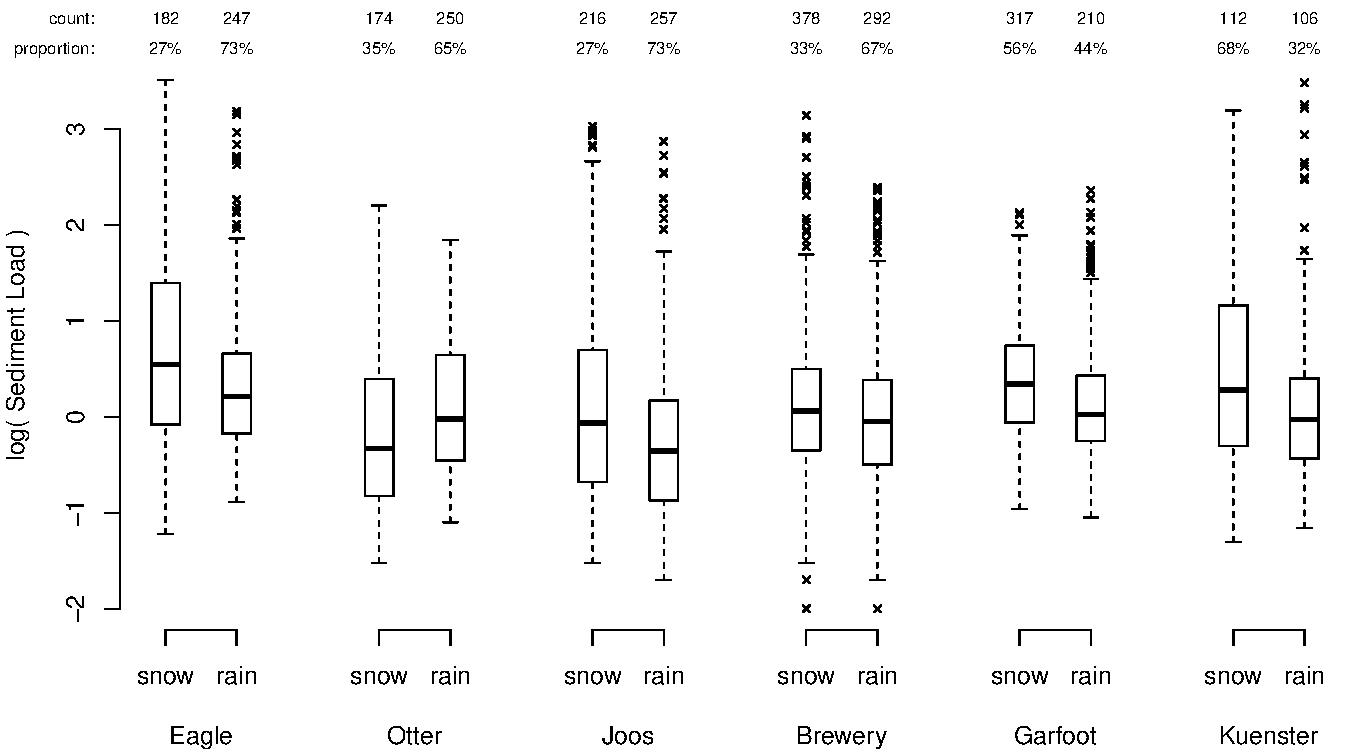
\includegraphics{loadings-boxplot_stot}
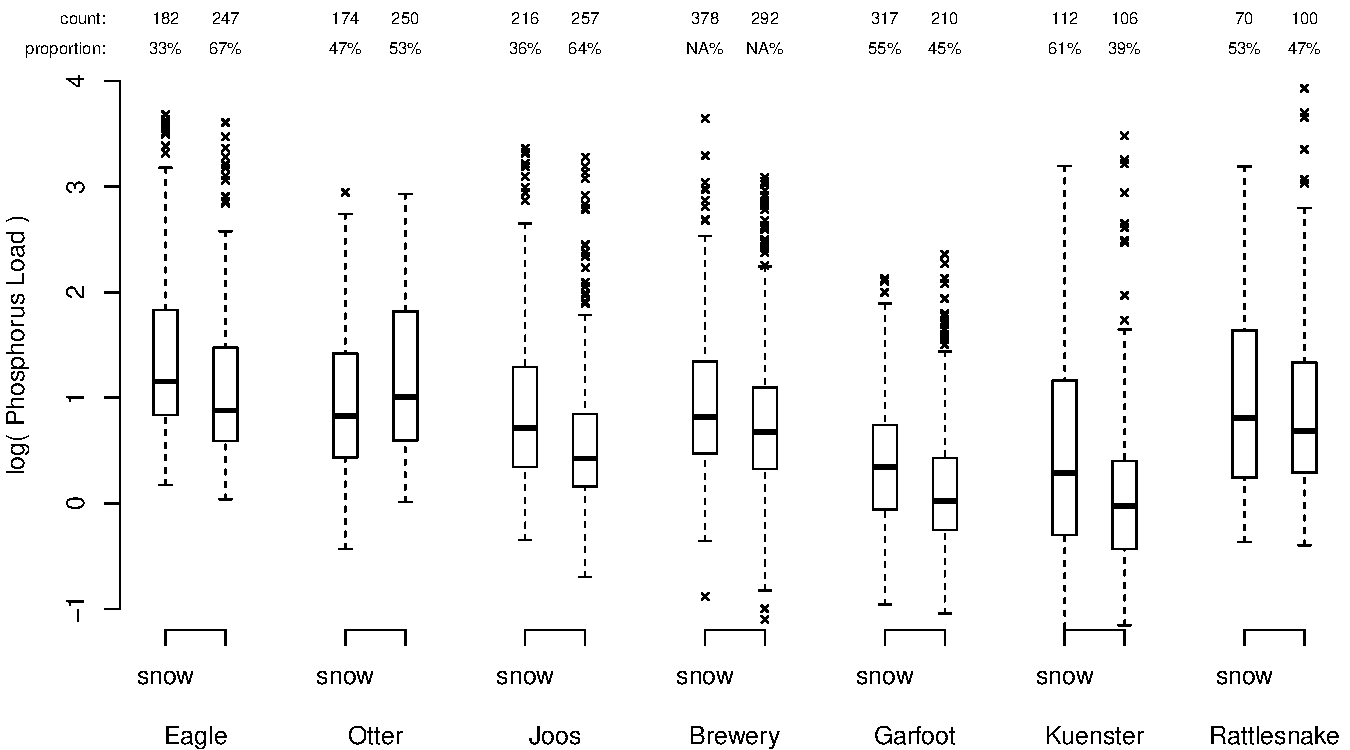
\includegraphics{loadings-boxplot_ptot}
    \end{center}
\end{figure}










\begin{figure}
    \begin{center}
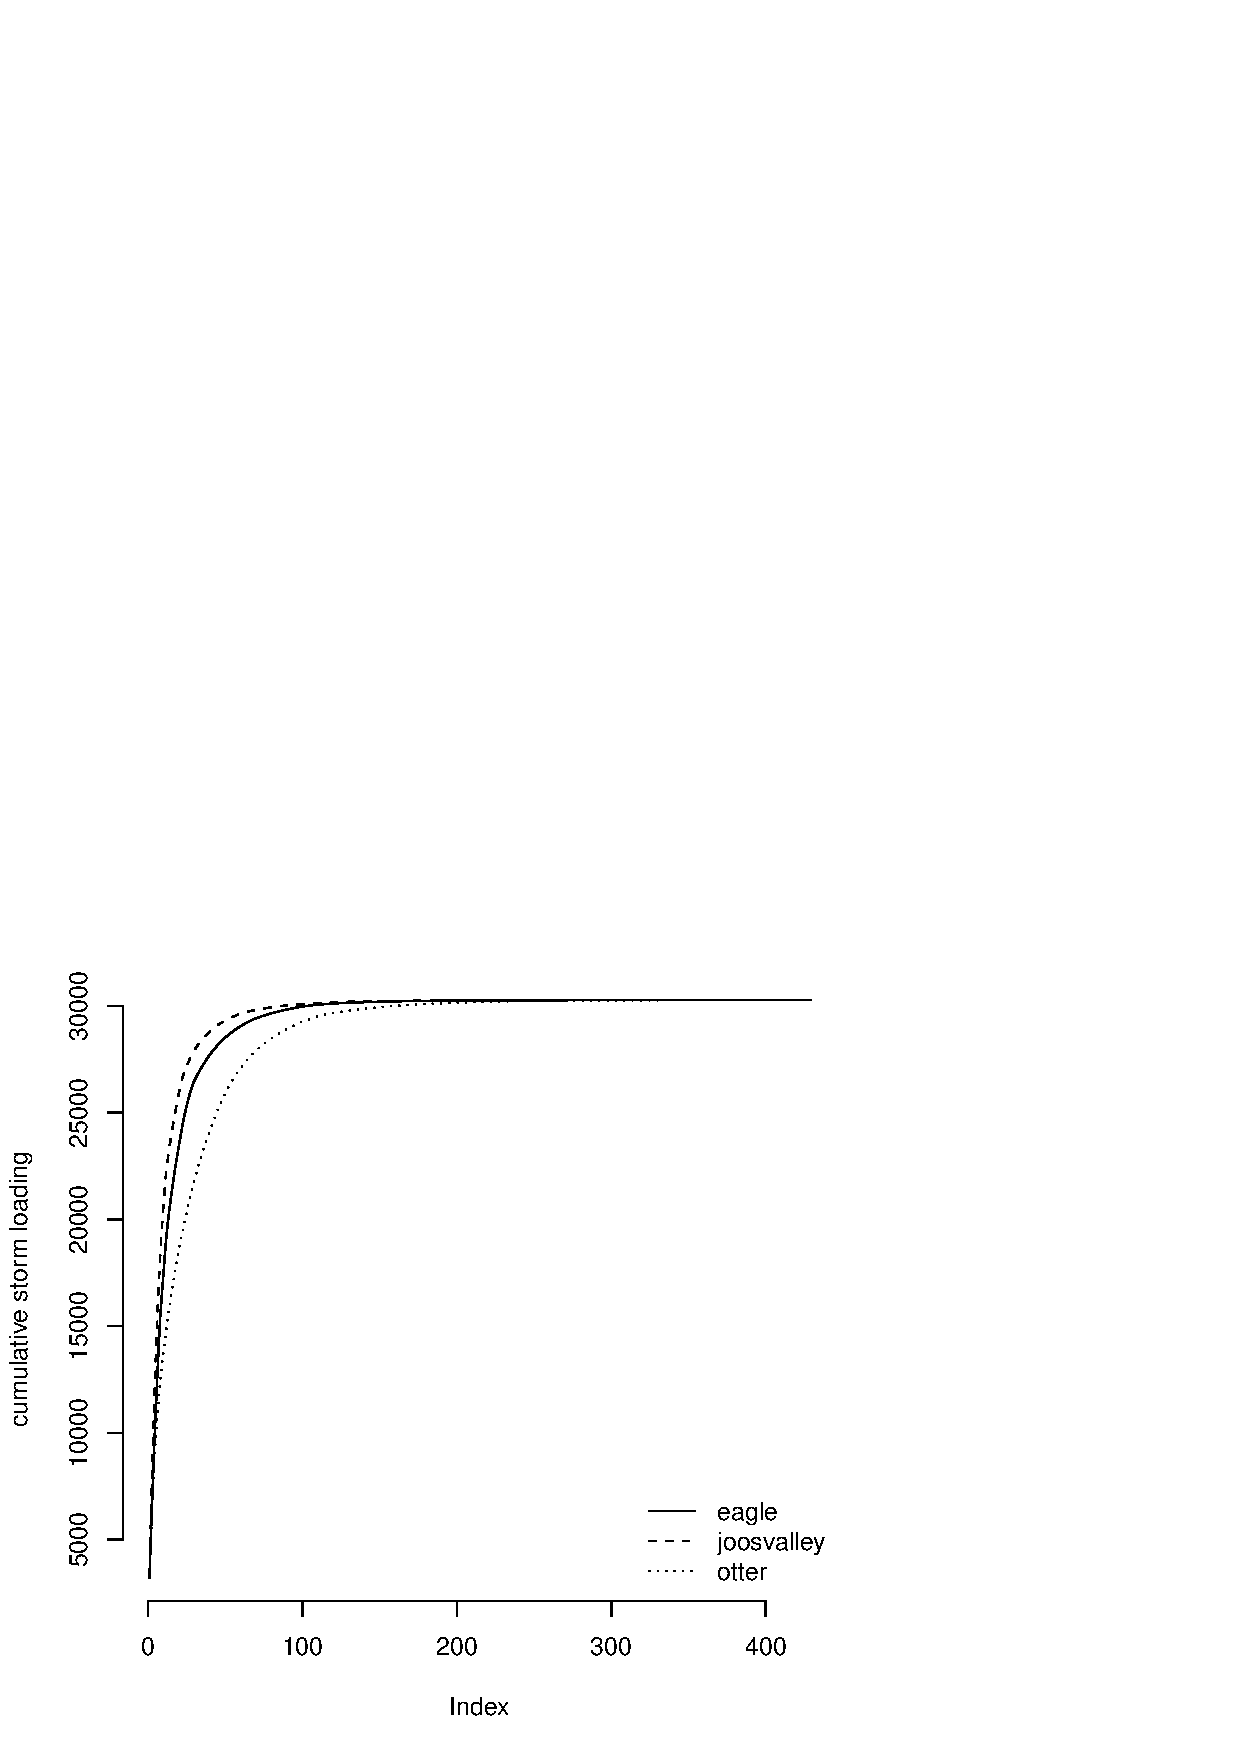
\includegraphics{loadings-figure1}
    \end{center}
    \caption{Cumulative storm loadings at the three creeks.\label{cdf}}
\end{figure}


\begin{figure}
    \begin{center}
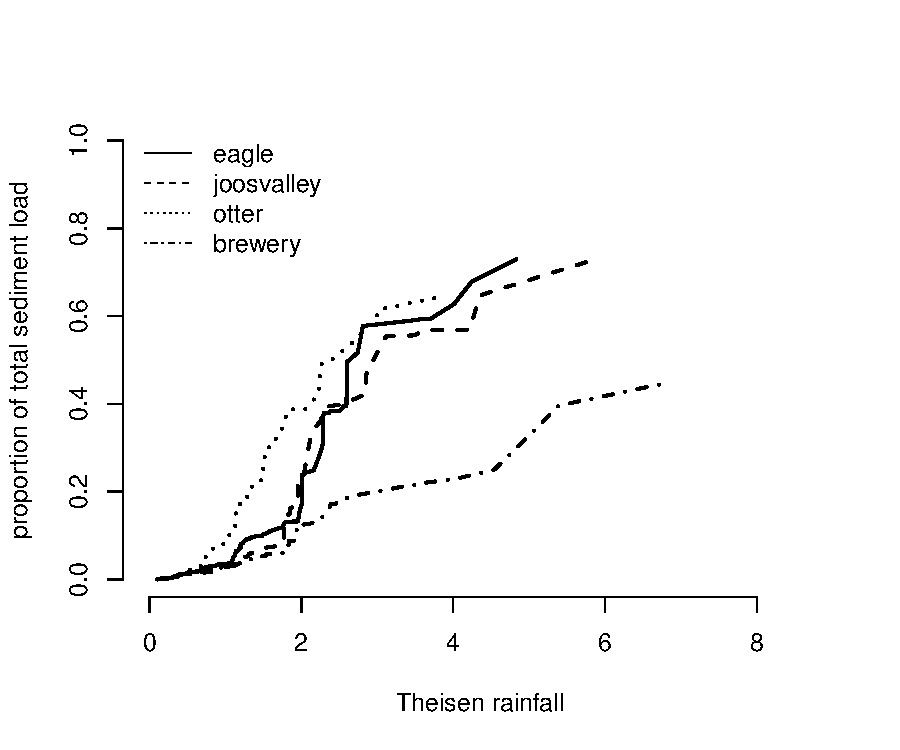
\includegraphics{loadings-figure2}
    \end{center}
    \caption{Proportion of the total sediment load contributed by rainfall events up to the size shown. Snowmelt-driven events are excluded.\label{cdf-p}}
\end{figure}

\begin{figure}
    \begin{center}
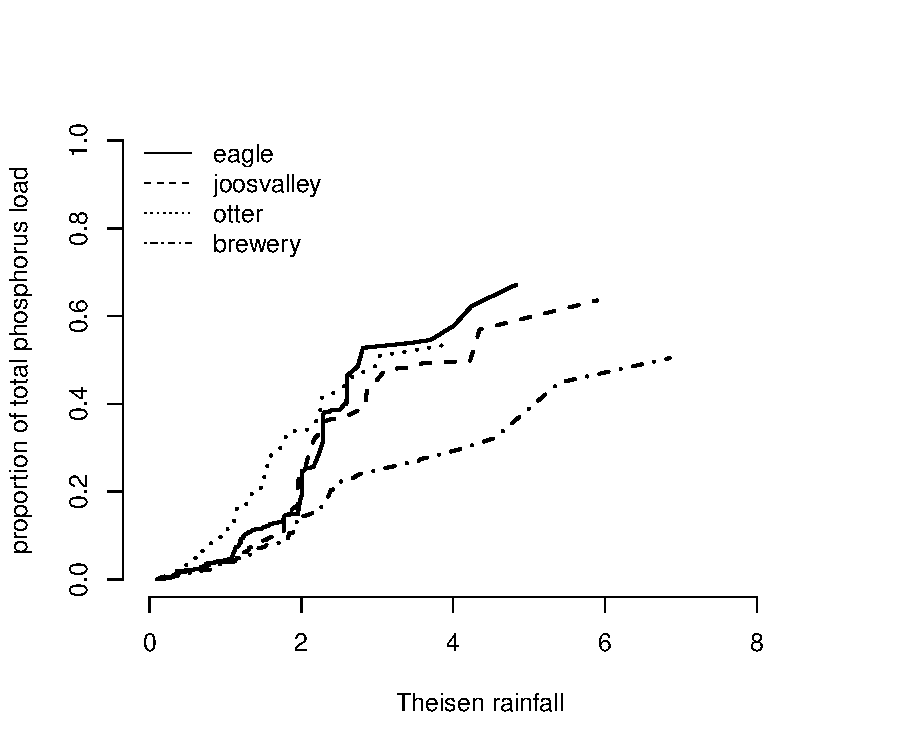
\includegraphics{loadings-figure3}
    \end{center}
    \caption{Proportion of the total phosphorus load contributed by rainfall events up to the size shown. Snowmelt-driven events are excluded.\label{cdf-s}}
\end{figure}



Figure out what proportion of total sediment loading is contributed by the top 10\% of storms:\\








\section{Data}

\paragraph{Description}
The data in this report comes from four Wisconsin streams that were monitored (with some gaps in data collection) between 1989 and 2007. The streams and the period during which each was monitored are:

\begin{table}[h]
    \begin{tabular}{r l}
        \textbf{Stream} & \textbf{Monitored} \\
        Eagle & 1991-1994, 2003-2007\\
        Joos Valley & 1990-1994, 2002-2007\\
        Otter & 1990-1997, 2000-2002\\
        Brewery & 1989, 1994-2002, 2004-2005\\
    \end{tabular}
\end{table}

Each entry in our data set represents one ``loading event", which is defined based on the hydrograph - the event begins when the loading rises from a base level toward a peak, and ends when the loading falls back to its new base level. Two kinds of load are measured for each event - the sediment load and the phosphorus load. There are two typical ways that sediment and phosphorus get into streams - they can be carried either by runoff during a rainstorm or by melting snow.\\

Not all of the data can be collected for each event. For instance, rainfall is measured only when the ground is free of snow because snow interferes with the rain gauges. And the amount of snowmelt is estimated by multiplying the water content of the snow by the change in snow depth a warm snap, which is inaccurate when additional snow falls during that event. Broadly, there is one set of measurements that are made during rainfall-driven events and a different set of measurements that are made during snowmelt-driven events. Because of this, the two types of event are modeled separately.\\

Within the category of events that are driven by rainfall, we investigate making a further split (on May 15 each year) between ``early post-snow" and ``late post-snow" events. Erosion may be more common early in the spring, before most of the summer's vegetation appears, which would alter the relationship between our inputs and outputs. See the Modeling section for further discussion of this split.\\

\paragraph{Exploratory Analysis}
Our anaysis targets the phosphorus and sediment loads carried by each stream. Using ``Rainmaker" software, each load can be broken into two parts: base load and storm load. We will consider models of the storm load and of the total load.\\

Over the course of the monitoring period, the majority of the total load (both of sediment and of phosphorus) was carried during just a few major events. Just 10\% of the events carried between 0\% (at Eagle) and 0\% (at Eagle) of the total sediment load and 0\% (at Eagle) and 0\% (at Eagle) of the total phosphorus load.\\

Table \ref{proportion_of_majors} shows that the major loading events that produce the majority of the loading can be occur during each of the three annual periods. However, the events caused by snowmelt produced a smaller proportion of major events than their proportion of all events, and their relative contribution to the total sediment load was smaller than their proportion of loading events. So while snowmelt \emph{can} cause a major loading event, a snowmelt-driven event is less likely to be a major event than is one driven by rainfall.\\


\begin{table}[h]
    \begin{center}
    \begin{tabular}{lr|lr|lr|l}
        & \multicolumn{2}{c}{Snowmelt    }\ & \multicolumn{2}{c}{Early post-snow}\ & \multicolumn{2}{c}{Late post-snow} \\
        Creek & All & Major & All & Major & All & Major \\
        \hline 
        Eagle & 42\% & 30\% & 13\% & 19\% & 45\% & 51\% \\
        Otter & 41\% & 42\% & 11\% & 19\% & 48\% & 40\% \\
        Joos & 46\% & 31\% & 11\% & 17\% & 43\% & 52\% \\
        
        Brewery & 56\% & 52\% & 6\% & 6\% & 38\% & 42\% \\
        
    \end{tabular}
    \end{center}
    \caption{Each pair of columns represents one of the three annual periods. The column on the left of each pair is the proportion of all events in the study that occured during this period; the column on the right is the proportion of major events that occured during this period. \label{proportion_of_majors}}
\end{table}



\begin{table}[h]
    \begin{center}
    \begin{tabular}{lrl}
    \textbf{Sediment} & $R^2$ & Model terms \\
    \hline
    Eagle & 0.503 & theisen\\
    & 0.755 & theisen + antecedent\_qbase\\
    & 0.767 & theisen + antecedent\_qbase + p15max\\
    & 0.773 & theisen + antecedent\_qbase + p15max + p60max\\
    
    Joos & & \\
    & 0.49 & theisen\\
    & 0.665 & theisen + antecedent\_qbase\\
    & 0.692 & theisen + antecedent\_qbase + p15max\\
    & 0.713 & theisen + antecedent\_qbase + p15max + ap\_2day\\

    Otter & & \\
    & 0.486 & theisen\\
    & 0.738 & theisen + antecedent\_qbase\\
    & 0.764 & theisen + antecedent\_qbase + antecedent\_tmean\\
    & 0.773 & theisen + antecedent\_qbase + antecedent\_tmean + julian\\

    Brewery & & \\
    & 0.433 & theisen\\
    & 0.459 & theisen + p30max\\
    & 0.51 & theisen + p30max + tmean
    \vspace{6mm}\\

    \textbf{Phosphorus} & $R^2$ & Model terms \\
    \hline
    Eagle & 0.579 & theisen\\
    & 0.783 & theisen + antecedent\_qbase\\
    & 0.784 & theisen + antecedent\_qbase + tmean\\
    & 0.793 & theisen + antecedent\_qbase + tmean + tmax\\
    
    Joos & & \\
    & 0.543 & theisen\\
    & 0.715 & theisen + antecedent\_qbase\\
    & 0.733 & theisen + antecedent\_qbase + p15max\\
    & 0.755 & theisen + antecedent\_qbase + p15max + ap\_2day\\

    Otter & & \\
    & 0.483 & theisen\\
    & 0.737 & theisen + antecedent\_qbase\\
    & 0.762 & theisen + antecedent\_qbase + tmean\\
    & 0.77 & theisen + antecedent\_qbase + tmean + julian\\

    Brewery & & \\
    & 0.602 & theisen\\
    & 0.641 & theisen + p30max\\
    & 0.674 & theisen + p30max + tmean\\

    \end{tabular}
    \end{center}
\end{table}







\begin{table}[h]
    \begin{center}
    \begin{tabular}{llccccc}
        &  &  & \multicolumn{2}{c}{Sediment} & \multicolumn{2}{c}{Phosphorus} \\
        Creek & Period & All events & Major events & Loading & Major events & Loading \\
        \hline 
        \multirow{3}{*}{Aggregated} & Snowmelt & 
        48\% &
        28\% & 
        40\% & 
        39\% & 
        48\% \\
        & Early post-snow & 
        10\% &
        23\% & 
        14\% & 
        17\% & 
        13\% \\
        & Late post-snow & 
        43\% &
        49\% & 
        46\% & 
        44\% & 
        39\% \\
        
        \hline 
        \multirow{3}{*}{Eagle} & Snowmelt & 
        42\% &
        27\% & 
        30\% & 
        33\% & 
        37\% \\
        & Early post-snow & 
        13\% &
        29\% & 
        19\% & 
        23\% & 
        21\% \\
        & Late post-snow & 
        45\% &
        44\% & 
        51\% & 
        44\% & 
        42\% \\
        
        \hline 
        \multirow{3}{*}{Joos} & Snowmelt & 
        46\% &
        27\% & 
        31\% & 
        36\% & 
        35\% \\
        & Early post-snow & 
        11\% &
        20\% & 
        17\% & 
        17\% & 
        19\% \\
        & Late post-snow & 
        43\% &
        53\% & 
        52\% & 
        47\% & 
        46\% \\
        
        \hline 
        \multirow{3}{*}{Otter} & Snowmelt & 
        41\% &
        35\% & 
        42\% & 
        47\% & 
        58\% \\
        & Early post-snow & 
        11\% &
        20\% & 
        19\% & 
        17\% & 
        12\% \\
        & Late post-snow & 
        48\% &
        44\% & 
        40\% & 
        37\% & 
        30\% \\
        
        \hline 
        \multirow{3}{*}{Brewery} & Snowmelt & 
        56\% &
        33\% & 
        52\% & 
        50\% & 
        60\% \\
        & Early post-snow & 
        6\% &
        5\% & 
        6\% & 
        5\% & 
        4\% \\
        & Late post-snow & 
        38\% &
        63\% & 
        42\% & 
        46\% & 
        37\% \\
    \end{tabular}
    \end{center}
\end{table}



 %\begin{landscape}
 \begin{center}
\psset{linecolor=black,tnsep=2pt,tnheight=0cm,treesep=.3cm,levelsep=40pt,radius=10pt}
%     \def\psedge#1#2{\ncangle{#2}{#1}}
%     \pstree[treemode=R]
    \Tcircle[fillcolor=yellow,fillstyle=solid]{ 1 }~{\textit{48.34}}
 \end{center}
GUIDE piecewise constant least-squares regression tree model.
At each intermediate node, a case goes to the left branch 
  if and only if the condition is satisfied.
Number in italics beneath leaf node is sample mean of stottot.
 %\end{landscape} %\begin{landscape}
 \begin{center}
\psset{linecolor=black,tnsep=2pt,tnheight=0cm,treesep=.3cm,levelsep=40pt,radius=10pt}
%     \def\psedge#1#2{\ncangle{#2}{#1}}
%     \pstree[treemode=R]
  \pstree{\Tcircle{ 1 }~[tnpos=l]{\shortstack[r]{nwsprec\\$\leq$ 1.91}}}{
    \Tcircle[fillcolor=yellow,fillstyle=solid]{ 2 }~{\textit{22.17}}
    \Tcircle[fillcolor=yellow,fillstyle=solid]{ 3 }~{\textit{1401.91}}
 }
 \end{center}
GUIDE piecewise constant least-squares regression tree model.
At each intermediate node, a case goes to the left branch 
  if and only if the condition is satisfied.
Number in italics beneath leaf node is sample mean of stottot.
 %\end{landscape} %\begin{landscape}
 \begin{center}
\psset{linecolor=black,tnsep=2pt,tnheight=0cm,treesep=.3cm,levelsep=40pt,radius=10pt}
%     \def\psedge#1#2{\ncangle{#2}{#1}}
%     \pstree[treemode=R]
  \pstree{\Tcircle{ 1 }~[tnpos=l]{\shortstack[r]{theisen\\$\leq$ 2.20}}}{
  \pstree{\Tcircle{ 2 }~[tnpos=l]{\shortstack[r]{totalwater\\$\leq$ 1.98}}}{
    \Tcircle[fillcolor=yellow,fillstyle=solid]{ 4 }~{\textit{18.05}}
    \Tcircle[fillcolor=yellow,fillstyle=solid]{ 5 }~{\textit{272.43}}
   }
    \Tcircle[fillcolor=yellow,fillstyle=solid]{ 3 }~{\textit{578.23}}
 }
 \end{center}
GUIDE piecewise constant least-squares regression tree model.
At each intermediate node, a case goes to the left branch 
  if and only if the condition is satisfied.
Number in italics beneath leaf node is sample mean of stottot.
 %\end{landscape}



\section{Analysis}

\paragraph{Variable selection} In order to make a model of the load carried by the stream, we need to select the predictor variables that have explanatory power. We use stepwise regression with the Bayesian Information Criterion (BIC) to screen the potential predictor variables.

\begin{table}[h]
    \begin{center}
    \begin{tabular}{ll}
        \textbf{Solids} & \\
        \hspace{5mm} Eagle: & theisen, antecedent\_qbase, p15max, p60max\\
        \hspace{5mm} Joos: & theisen, antecedent\_qbase, p15max, ap\_2day\\
        \hspace{5mm} Otter: & theisen, antecedent\_qbase, antecedent\_tmean, julian\\
        \hspace{5mm} Brewery: & theisen, p30max, tmean
    \vspace{2mm}\\
        \textbf{Phosphorus} & \\
        \hspace{5mm} Eagle: & theisen, antecedent\_qbase, tmean, tmax, p15max, p30max\\
        \hspace{5mm} Joos: & theisen, antecedent\_qbase, p15max, ap\_2day\\
        \hspace{5mm} Otter: & theisen, antecedent\_qbase, tmean, julian\\
        \hspace{5mm} Brewery: & theisen, p30max, tmean, ap\_3day\\
    \end{tabular}
    \end{center}
\end{table}


%\begin{table}[h]
%    \begin{center}
%    \begin{tabular}{lrl}
%        Solids: & & \\
%        & Eagle & theisen, antecedent_qbase, p15max, p60max\\
%        & Joos & theisen, antecedent_qbase, p15max, ap_2day\\
%        & Otter & theisen, antecedent_qbase, antecedent_tmean, julian\\
%        & Brewery & theisen, p30max, tmean\\
%        \hline \\
%        Phosphorus: & & \\
%        & Eagle & theisen, antecedent_qbase, tmean, tmax, p15max, p30max\\
%        & Joos & theisen, antecedent_qbase, p15max, ap_2day\\
%        & Otter & theisen, antecedent_qbase, tmean, julian\\
%        & Brewery & theisen, p30max, tmean, ap_3day\\
%    \end{tabular}
%    \end{center}
%\end{table}




\bibliographystyle{plain}
\bibliography{../../references/bibliography}

\end{document}
